\documentclass[10pt,a5paper,english,hidelinks]{article}
\usepackage{arev}
\usepackage[T1]{fontenc}
\usepackage[utf8]{inputenc}
\usepackage{babel}
\usepackage[a5paper, margin=1.25cm]{geometry}
\usepackage{multicol}
\usepackage{listings}
\usepackage{graphicx}
\usepackage{tabularx}
\usepackage[most]{tcolorbox}
\usepackage{capt-of}
\usepackage{hyperref}
\usepackage{longtable}
\usepackage[font={footnotesize,bf},labelfont=bf]{caption}
\usepackage{booktabs}
\usepackage{tocloft}
\usepackage{tabu}
\usepackage{tikz}
\usepackage[justification=centering]{caption}
\usepackage{catchfilebetweentags}
\usetikzlibrary{calc}




\setlength{\columnseprule}{0.4pt}
\setlength\parindent{0pt}

% =================================================================================================
\newtcolorbox{ImportantBox}[2][]{enhanced,
    fonttitle=\ttfamily,
    fontupper=\ttfamily,
    sharp corners,
		leftrule=1mm,
		rightrule=0.25mm,
		bottomrule=0.25mm,
		toprule=0.25mm,
    colback=white,
    colbacktitle=white,
    coltitle=black,
    boxed title style={colframe=white},
    attach boxed title to top center={yshift=-5.5mm}, 
    title=#2,#1}
\newenvironment{IMPORTANT}[1][]
{
	\begin{ImportantBox}{\tikz{\node at (0,-.5) {
\includegraphics[height=0.5cm]{../includes/icon_important.png}}}}
	\begin{minipage}{\textwidth}
}
{
\end{minipage}
\end{ImportantBox}
}

% =================================================================================================
\newenvironment{USEFUL}[1][]
{
	\begin{ImportantBox}{\tikz{\node at (0,-.5) {
\includegraphics[height=0.6cm]{../includes/icon_info.png}}}}
	\begin{minipage}{\textwidth}
}
{
\end{minipage}
\end{ImportantBox}
}

% =================================================================================================
\newenvironment{BUG}[1][]
{
	\begin{ImportantBox}{\tikz{\node at (0,-.5) {
\includegraphics[height=0.6cm]{../includes/icon_bug.png}}}}
	\begin{minipage}{\textwidth}
}
{
\end{minipage}
\end{ImportantBox}
}

% =================================================================================================

\begin{document}

\clearpage
\begin{titlepage}

\begin{center}
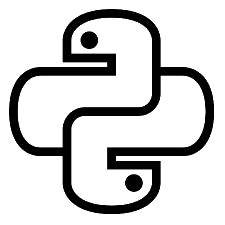
\includegraphics[height=1.25cm]{../includes/icon_main.png}\\
\vspace*{6cm}%
\textbf{\Huge quickdoxy}\\
\vspace*{0.25cm}%	
\textbf{\huge User Manual}\\
\vspace*{8.5cm}%
\end{center}

\begin{flushright}
	\mbox{\scriptsize
	\lstinputlisting{about.info}
	}
\end{flushright}
\end{titlepage}
\thispagestyle{empty}
%\begin{multicols}{2}
\begin{flushleft}
\emph{Preface}
\end{flushleft}


\textit{quickdoxy} provides a graphical wrapper around a portable doxygen distribution. It can be used to extract a copy of that 
distribution on any win64 machine, and to quickly create documentation of existing code. 

\textit{quickdoxy} does not provide means for detailed parameterization of the doxygen run/output. However, any parameterization
done in the config files of the extracted doxygen distribution will be taken into account when running \textit{quickdoxy}.
\begin{flushleft}

-- --

\end{flushleft}

\noindent Within this document, the following keywords and symbols are used to \mbox{emphasise} certain information:
\begin{IMPORTANT}
Information on limitations of the software, background knowledge, and user interactions that may damage existing files on the computer.
\end{IMPORTANT}
\begin{USEFUL}
Insightful information on how to use \textit{quickdoxy} to its full potential.
\end{USEFUL}		
\begin{BUG}
Known bug or issue that must be worked around.
\end{BUG}			
\addtocounter{page}{-1}
\newpage	
%\end{multicols}
		
\tableofcontents
\thispagestyle{empty}
\addtocounter{page}{-1}
\newpage		

\section{Setup} %==================================================================================

\textit{quickdoxy} is distributed as either a .exe file, or a .pyw python file. The
.exe will run on any 64 bit windows machine without any further setup required.

The .pyw file can be executed by calling \texttt{pythonw quickdoxy.py} from the command line or by double-clicking, 
if python is installed on the system and all required modules are present. Since the GUI requires \textit{pyQt5}, 
a convenient way to make sure that the requirements are met is to use the \textit{Anaconda} distribution (Version  $\geq$ 5)\footnote{https://www.anaconda.com/download/}.
If Anaconda is installed, the only module that must be added manually is \textit{configargparse}\footnote{call \texttt{pip install configargparse} from an administrator command prompt}.

To build \textit{quickdoxy} from sources, make sure that in addition to the dependencies above, the following software is present on the system:
\begin{itemize}
	\item \textit{pyinstaller}, a tool to create .exe files from python scripts\footnote{call \texttt{pip install pyinstaller} from an administrator command prompt},
	\item \textit{pyuic5}, used to convert Qt .ui-sources into python modules,
	\item \textit{pyrcc5}, to convert Qt-resource files into python modules,
	\item \textit{pdf\LaTeX} (e.g. \textit{MikTex} $\geq$ 2.9) to compile the documentation.
\end{itemize}

\textit{quickdoxy} uses permanent settings that are stored in the registry. You can find them at\\
\texttt{Computer\textbackslash HKEY\_CURRENT\_USER \textbackslash Software \textbackslash HDRD \textbackslash quickdoxy}

\section{GUI overview} % ==========================================================================
\begin{center}
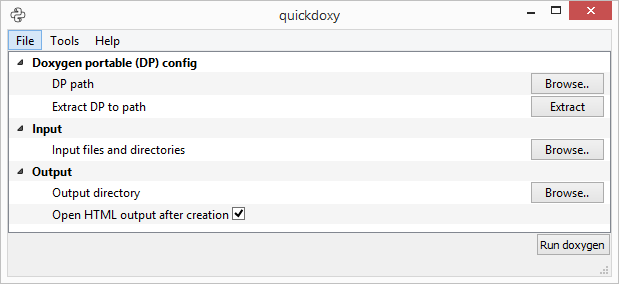
\includegraphics[width=.5\textwidth]{../includes/GUI.png}
\captionof{figure}{quickdoxygui}
\label{fig:quickdoxygui}
\end{center}

The GUI consists of a menu bar, the central parameter tree, and a status bar (see Figure \ref{fig:quickdoxygui}),

The program will give feedback to most user action via the program log. The last message in the log is always on display at the 
status bar on the bottom of the GUI. To open the full log, call \emph{Tools/toggle log} in the menu bar.

Calling \emph{File/Run Doxygen} or the corresponding button in the bottom right corner will call doxygen, using the
parameters provided in the parameter tree. If the parameters are not correct, doxygen is not called and an error is logged.

Calling \emph{Help/Documentation} opens this document, \\
and calling \emph{Help/About} displays build information in the log.

\bigbreak

In order to make a proper call to doxygen, the parameters in the parameter tree must be set up properly. The parameter 
\emph{Doxygen portable (DP) config / DP path} contains the path to the doxygen portable distribution that will be used. This
parameter is permanently stored in the registry and only needs to be set up once.
Before running \emph{quickdoxy} for the first time, select a path for doxygen portable and click 
\emph{Doxygen portable (DP) config / Extract DP to path}. This extracts all data needed into the selected directory.

The parameter \emph{Input / Input files and directories} specifies all inputs to doxygen. 
It may contain any number of files and/or directories, seperated by semicola.

The parameter \emph{Output / Iutput directory} specifies the directory where the results (HTML documentation \& \LaTeX documentation)
is stored. If the HTML documentation should be displayed after the build process has finished, check \emph{Output / Open HTML output after creation}.

\begin{USEFUL}
All parameters except the doxygen portable path can also be passed via command line, which allows quickdoxy to run in batch mode without showing the GUI.
See section \ref{sec:CommandLineInterface} for details.
\end{USEFUL}

\section{Running \textit{quickdoxy}}
To run \textit{quickdoxy} using the GUI, call the program (by double clicking, or from the command line),
extract doxygen portable, if needed, select Input files, output files and click the \emph{Run doxygen button}. 
By default, the resulting HTML-Documentation is opened as soon as the process finished.

To run quickdoxy from the command line, refer to section \ref{sec:CommandLineInterface}. In order to 
skip the GUI, the \texttt{-{}-batchmode} flag must be passed. If it is not passed, the GUI open and 
the values specified in the command line are entered in the parameter tree.

% =================================================================================================		
% autogenerated sections
\section{Shortcuts}
\label{sec:Shortcuts}
\begin{flushleft}\tiny\begin{longtabu} to \textwidth {|X[1,c,m]|X[8,l,m]|X[3,c,m]|X[12,c,m]|}
\caption{quickdoxy shortcuts}\label{tab:shortcuts}\endfirsthead
\caption*{Table \ref{tab:shortcuts} (continued)}\endhead
\hline
&\textbf{Name}&\textbf{Shortcut}&\textbf{Description}\\
\hline
\tikz[baseline=-0.1cm]{\node at (0,0) {
\includegraphics[height=0.25cm]{../includes/icon_info.png}}}&About&Shift+F1&displays version information\\
\hline
\tikz[baseline=-0.1cm]{\node at (0,0) {
\includegraphics[height=0.25cm]{../includes/icon_docu.png}}}&Documentation&F1&opens the documentation\\
\hline
\tikz[baseline=-0.1cm]{\node at (0,0) {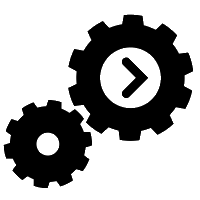
\includegraphics[height=0.25cm]{../includes/icon_run.png}}}&Run Doxygen&F2&Runs doxygen with the specified parameters\\
\hline
\tikz[baseline=-0.1cm]{\node at (0,0) {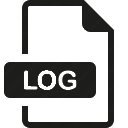
\includegraphics[height=0.25cm]{../includes/icon_log.png}}}&toggle log&Ctrl+L&opens / closes the log window\\
\hline
\end{longtabu}\end{flushleft}
\section{Command line interface}
\label{sec:CommandLineInterface}

\begin{center}
\lstinputlisting[basicstyle=\scriptsize]{cli_help.txt}
\end{center}
		
\listoffigures
% =================================================================================================
\end{document}
